%% sample file for Modelica 2015 Conference paper
%% Copyright 2015 DLR and the Modelica Association
%
% This work may be distributed and/or modified under the
% conditions of the LaTeX Project Public License, either version 1.3
% of this license or (at your option) any later version.
% The latest version of this license is in
%   http://www.latex-project.org/lppl.txt
% and version 1.3 or later is part of all distributions of LaTeX
% version 2005/12/01 or later.
%
% This work is 'maintained' on GitHub:
%   https://github.com/modelica-association/conference-templates
%
% The Current Maintainers are: @akloeckner, @dietmarw, @berhnard-thiele
%
% This work consists of all files in the GitHub repository except
% a) The files indicated by .gitignore files
% b) The GitHub management files .gitignore, *.md
%
% This class is created from the template for the Modelica 2015 conference

\documentclass{modelica}

\hypersetup{%
	pdftitle  = {Latex Template for the International Modelica Conference},
	pdfauthor = {Author Name1, Author Name2},
        pdfsubject = {11th International Modelica Conference 2015},
        pdfkeywords = {Modelica, conference, LaTeX, template},
	hidelinks,
	pdfpagelayout = SinglePage,
	pdfcreator = pdflatex,
	pdfproducer = pdflatex}


% begin the document
\begin{document}
\thispagestyle{empty}

\title{Int. Modelica Conf. 2015 Paper Title}
\author[1]{Author Name}
\author[1]{Author Name}
\author[2]{Author Name}
\affil[1]{Department, University, Country, {\small\texttt{\{name1,name2\}@university.org}}}
\affil[2]{Company, Country, {\small\texttt{name3@company}}}

% \title{\textbf{Int. Modelica Conf. 2015 Paper Title}}
% \author{{\large
% Author Name$^1$ \quad Author Name$^1$ \quad Author Name$^2$\vspace{2mm}\\
%   {}$^1$Department, University, Country, \textsf{\{name1,name2\}@university.org}\\
%   {}$^2$Company, Country, \textsf{name3@company}}


\date{} % <--- leave date empty
\maketitle\thispagestyle{empty} %% <-- you need this for the first page
\abstract{%
This template shows the guidelines on how to create a paper to be
submitted to the International Modelica Conference. Templates are
available for both the \LaTeX\ and Microsoft Word environment. This
particular template document should work with pdf\LaTeX\ which is a
\LaTeX\ variant which directly outputs PDF files instead of
postscript files. However, if required it can be adapted to be used
with a traditional \LaTeX\ document processor\footnote{Essentially by
replacing the PDF files \textsf{figure1.pdf} and
\textsf{figure2.pdf} by EPS files (Encapsulated PostScript
format).}. Please visit \href{https://github.com/modelica-association/conference-templates}{\url{https://github.com/modelica-association/conference-templates}} if there are any questions or suggestions regarding this template.
}

\noindent\emph{Keywords: keyword1, keyword2}

\section{Introduction}

In the following section, short style guidelines are given.

\subsection{Title and Authors}
Words should be capitalized in the title, e.g., ``This is an Example of
a Correct Title''.  The author information should at least include
name, affiliation (department, university, country). Addresses and
emails are optional but strongly recommended.


\subsection{Abstract and Keywords}

The abstract should be written as one paragraph. It is not recommended
to exceed 150 words.

Appropriate keywords describing the content of the paper should be
supplied as a comma separated list.

\subsection{Fonts}

For all standard body text \emph{Times New Roman} with regular font style, and font size 10.5pt should be used. To emphasize a text or a word, use \emph{italic font style}. For verbatim text embedded in running text, including code fragments, use the style {\small\texttt{texttt}} with font Courier New with size 9.5pt should be used (1pt smaller than running text)

For separate Modelica code examples, use the style font size 9~pt.  Similar for non-Modelica code examples. For formatting Modelica code this template used the listings definitions from \href{https://github.com/modelica-tools/listings-modelica}{\url{https://github.com/modelica-tools/listings-modelica}} (included in the package).

Example:

\begin{lstlisting}
while x<20 loop
  x := x+y*2;
end while;
\end{lstlisting}


\section{Figures}

Figures should be numbered and include a description text. All figures
should be referenced within the body text using the capitalized word
``Figure'' followed by the figure number. For example,
Figure~\ref{fig:figure1} shows a figure located inside one column and
Figure~\ref{fig:figure2} illustrates how a figure can span over two
columns.

\begin{figure}[b]
\centering
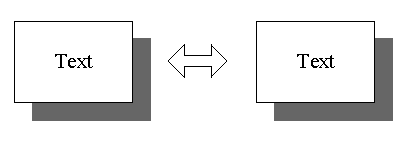
\includegraphics[width=0.4 \textwidth]{resources/figure1}
\caption{An example of a figure that fits into one column.}
\label{fig:figure1}
\end{figure}

\begin{figure*}[t]
\centering
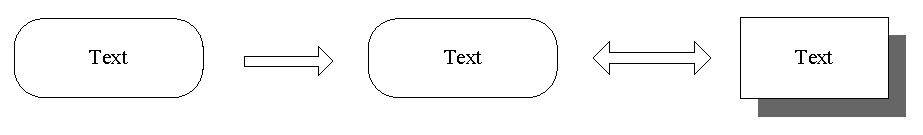
\includegraphics[width=0.9 \textwidth]{resources/figure2}
\caption{Another example of a figure that spans over two columns.}
\label{fig:figure2}
\end{figure*}

Table~\ref{tab:extab} illustrates the use of tables. It uses the
booktabs package which provides improved typesetting of tables.
\begin{table}[htbp]
  \caption{Sizes of compiler phases, lines of code.}\label{tab:extab}
  \centering
  \begin{tabular}{p{6cm}l} \toprule
      \emph{Compiler Phase} & \emph{Lines} \\
      \midrule
      BackEnd (from flat Modelica to sorted eq.syst.) & 29190 \\
      Code generation (generated code) & 35971 \\
      Code generation (template source code) & 8957 \\
      FrontEnd (up to flat Modelica) & 92192 \\
      OpenModelica scripting environment & 21883 \\
      Template language Susan compiler & 12119 \\
      Utility modules & 12983 \\
      \emph{Total size (excl.\ generated code)} & \emph{194218} \\
      \bottomrule
  \end{tabular}
\end{table}

\section{Equations}
Equations should be numbered on the right side, such as:
\begin{align}
a_1& =b_1+c_1\\
a_2& =b_2+c_2-d_2+e_2
\end{align}


\section{Bibliographic References}
The bibliographic reference list are shown at the end of the paper;
starting with an unnumbered heading \emph{``References''}. The list of
references should be sorted in alphabetic order according to the first
author's surname.

Citations are stated within the body text using the name of the
reference enclosed within parentheses, e.g., \citep{Pantelides:1988}. If
more than one reference is cited at the same place, the list should be
sorted, separated by semicolons and within parentheses, e.g.,
\citep{DuffReid:1978,Pierce:2002,Plotkin:1981}. If possible, it is
encouraged to use DOIs instead of URLs in the bibliography.


%--------------------------------------------------------------------------------
% References using bibtex
\bibliography{example-paper}

\end{document}
